

\documentclass{beamer}

\mode<presentation> {
	
	% The Beamer class comes with a number of default slide themes
	% which change the colors and layouts of slides. Below this is a list
	% of all the themes, uncomment each in turn to see what they look like.
	
	%\usetheme{default}
	%\usetheme{AnnArbor}
	%\usetheme{Antibes}
	%\usetheme{Bergen}
	%\usetheme{Berkeley}
	%\usetheme{Berlin}
	%\usetheme{Boadilla}
	%\usetheme{CambridgeUS}
	%\usetheme{Copenhagen}
	%\usetheme{Darmstadt}
	%\usetheme{Dresden}
	%\usetheme{Frankfurt}
	%\usetheme{Goettingen}
	%\usetheme{Hannover}
	%\usetheme{Ilmenau}
	%\usetheme{JuanLesPins}
	%\usetheme{Luebeck}
	\usetheme{Madrid}
	%\usetheme{Malmoe}
	%\usetheme{Marburg}
	%\usetheme{Montpellier}
	%\usetheme{PaloAlto}
	%\usetheme{Pittsburgh}
	%\usetheme{Rochester}
	%\usetheme{Singapore}
	%\usetheme{Szeged}
	%\usetheme{Warsaw}
	
	% As well as themes, the Beamer class has a number of color themes
	% for any slide theme. Uncomment each of these in turn to see how it
	% changes the colors of your current slide theme.
	
	%\usecolortheme{albatross}
	%\usecolortheme{beaver}
	%\usecolortheme{beetle}
	%\usecolortheme{crane}
	%\usecolortheme{dolphin}
	%\usecolortheme{dove}
	%\usecolortheme{fly}
	%\usecolortheme{lily}
	%\usecolortheme{orchid}
	%\usecolortheme{rose}
	%\usecolortheme{seagull}
	%\usecolortheme{seahorse}
	%\usecolortheme{whale}
	%\usecolortheme{wolverine}
	
	%\setbeamertemplate{footline} % To remove the footer line in all slides uncomment this line
	%\setbeamertemplate{footline}[page number] % To replace the footer line in all slides with a simple slide count uncomment this line
	
	%\setbeamertemplate{navigation symbols}{} % To remove the navigation symbols from the bottom of all slides uncomment this line
}

\usepackage{graphicx} % Allows including images
\usepackage{booktabs} % Allows the use of \toprule, \midrule and \bottomrule in tables

%----------------------------------------------------------------------------------------
%	TITLE PAGE
%----------------------------------------------------------------------------------------

\title[Conan]{Finding missing people
} % The short title appears at the bottom of every slide, the full title is only on the title page

%\author{Mohamed Atta} % Your name
\institute[CSE] % Your institution as it will appear on the bottom of every slide, may be shorthand to save space
{Supervisor: Dr.  Mahmoud Khalil\\
	Department of Computer and Systems Engineering\\
	Faculty of Engineering at Ain Shams University \\ % Your institution for the title page
	\medskip
	\textit{} % Your email address
}
\date{\today} % Date, can be changed to a custom date

\begin{document}
	
	\begin{frame}
		\titlepage % Print the title page as the first slide
	\end{frame}
	
	\begin{frame}
		\frametitle{Overview} % Table of contents slide, comment this block out to remove it
		\tableofcontents % Throughout your presentation, if you choose to use \section{} and \subsection{} commands, these will automatically be printed on this slide as an overview of your presentation
	\end{frame}
	
	
	\begin{frame}
		\frametitle{Team Names}
		\begin{center}
			Mohamed Atta Ibrahim \\Mohamed Yasser Ahmed
			\\Mahmoud Mohamed Benyamin\\ Hady Ashraf Ragab\\Yousef Abdelbadea Ali
			\vspace{2mm}
		\end{center}
	\end{frame}
	
	
	
	
	%----------------------------------------------------------------------------------------
	%	PRESENTATION SLIDES
	%----------------------------------------------------------------------------------------
	
	%------------------------------------------------
	\section{CONAN} % Sections can be created in order to organize your presentation into discrete blocks, all sections and subsections are automatically printed in the table of contents as an overview of the talk
	%------------------------------------------------
	
	\subsection{Detailed analysis}
	\subsection{Face recognition}
	\subsection{System architecture}
	\subsection{distance}
	\subsection{database design}


	
	\begin{frame}
		\frametitle{Introduction
		}
	In this project the user can find missing people by search with the old pictures
	or young pictures of missing people. The project uses techniques that extract
	features from the pictures and check similarity between the query picture and
	the pictures in the dataset to retrieve the similar picture to the query picture.
	\begin{figure}[H]
		\centering
		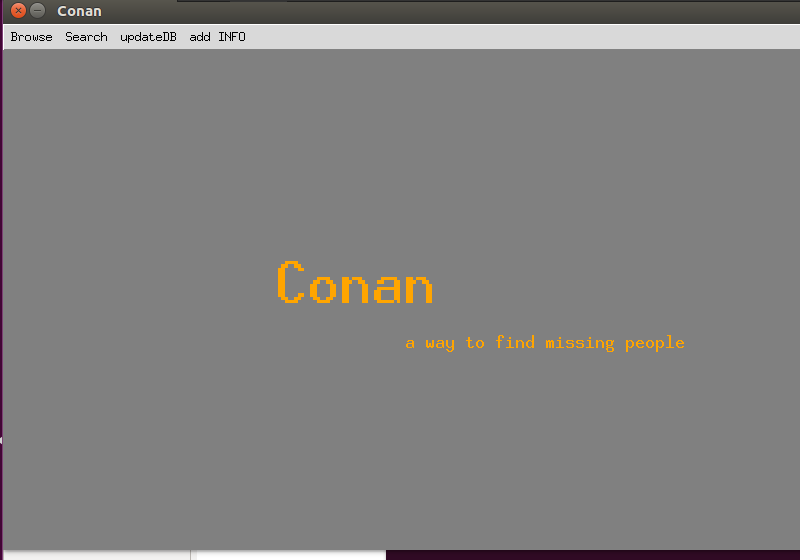
\includegraphics[width=120mm,height=60mm]{fig/00.png}
		%\caption{color histogram similarity measure }
		%\label{color histogram similarity measure}
	\end{figure}
	\end{frame}
\begin{frame}
	\frametitle{Detailed analysis}
		\begin{figure}[H]
		\centering
		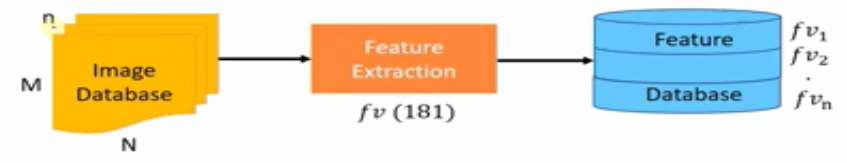
\includegraphics[width=120mm,height=25mm]{fig/21.png}
		%\caption{color histogram similarity measure }
		%\label{color histogram similarity measure}
	\end{figure}
	\begin{figure}[H]
	\centering
	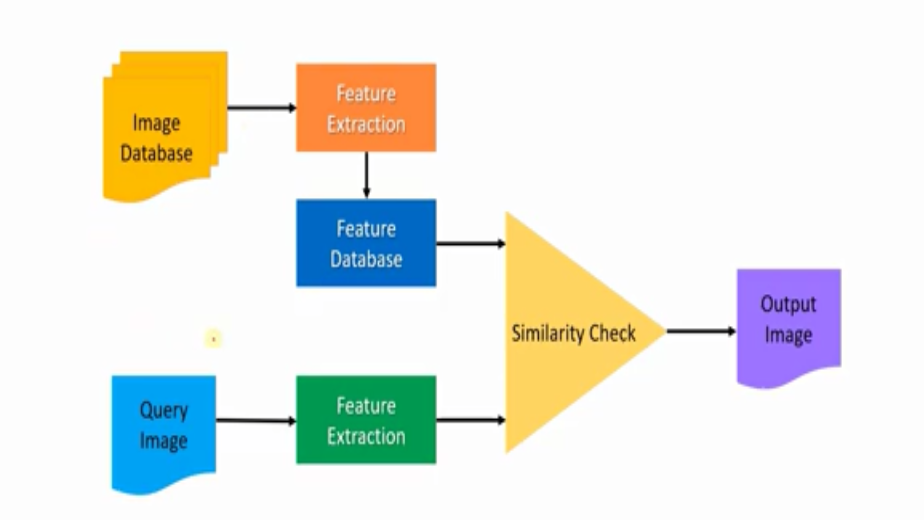
\includegraphics[width=120mm,height=50mm]{fig/19.png}
	%\caption{color histogram similarity measure }
	%\label{color histogram similarity measure}
\end{figure}
\end{frame}
\begin{frame}
	\frametitle{cont}
		\begin{figure}[H]
		\centering
		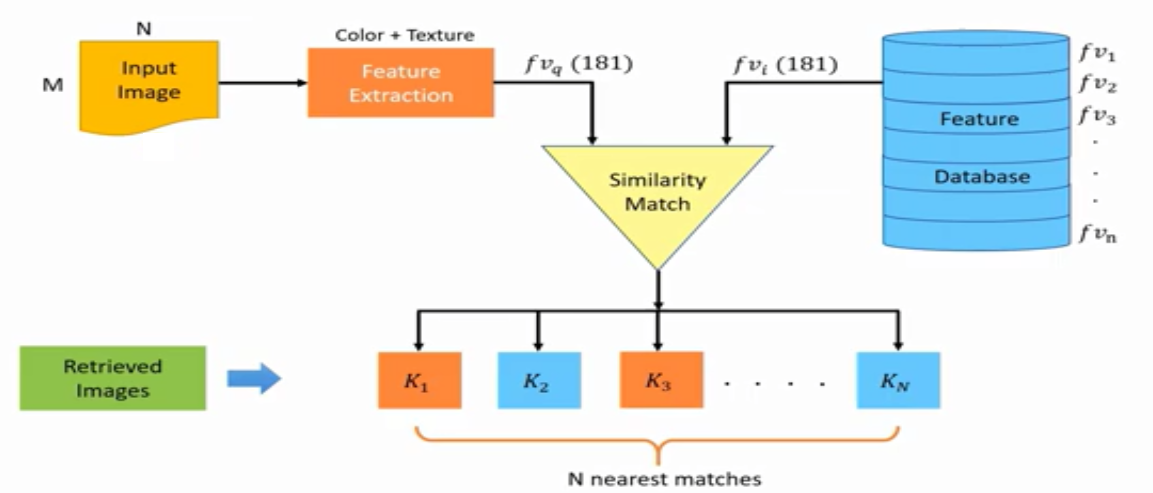
\includegraphics[width=120mm,height=60mm]{fig/20.png}
		%\caption{color histogram similarity measure }
		%\label{color histogram similarity measure}
	\end{figure}
\end{frame}
	
	\begin{frame}
		\frametitle{Face recognition}
			\begin{figure}[H]
			\centering
			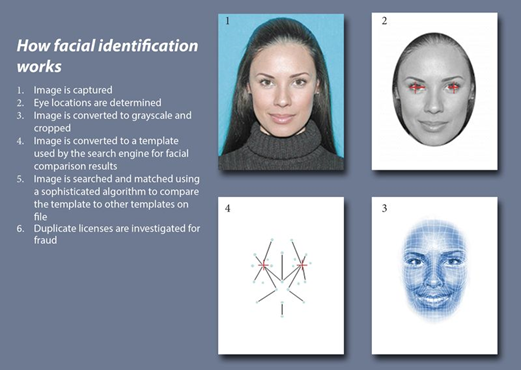
\includegraphics[width=120mm,height=60mm]{fig/30.png}
			%\caption{color histogram similarity measure }
			%\label{color histogram similarity measure}
		\end{figure}
	\end{frame}
\begin{frame}
	\frametitle{System architecture}
		\begin{figure}[H]
		\centering
		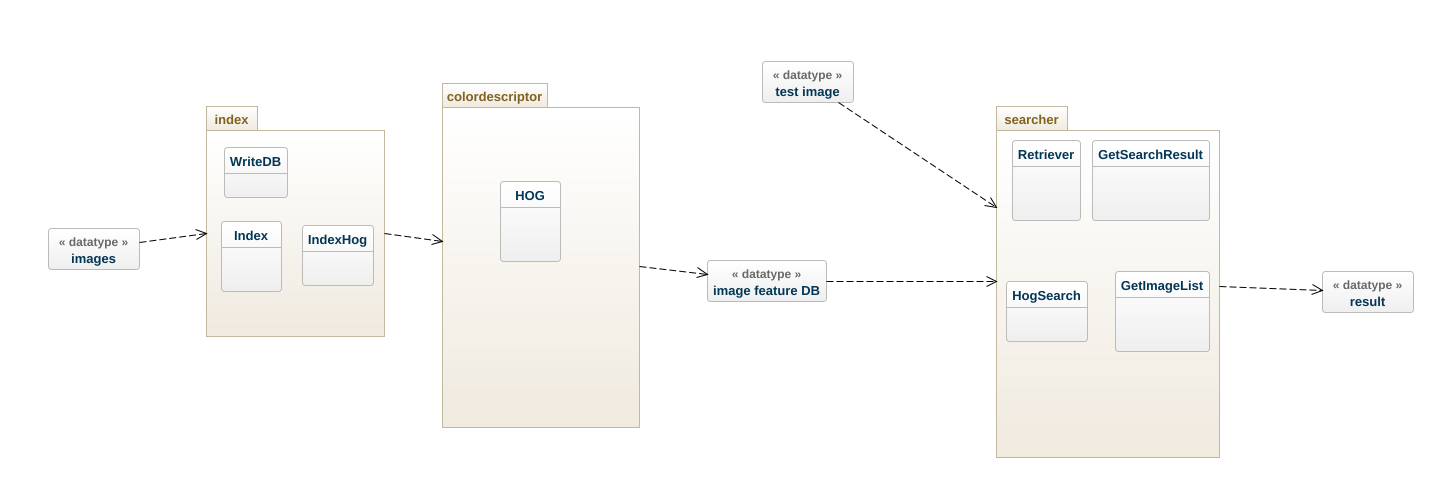
\includegraphics[width=120mm,height=60mm]{fig/22.png}
		%\caption{color histogram similarity measure }
		%\label{color histogram similarity measure}
	\end{figure}
\end{frame}
	\begin{frame}
		\frametitle{distance}
		we use Mean squared error method to compare between the image we search for
		and images saved in database
		\begin{itemize}
			\item Absolute Distance \\
			\begin{equation}
				D_{Absolute}(h,\bar{h})= \sum_{K-1}^{K} |h_{K}-\bar{h_{K}}|
			\end{equation}
			\item Euclidean Distance \\
			\begin{equation}
				D_{Euclidean}(h,\bar{h})= \sqrt{\sum_{K-1}^{K} (h_{K}-\bar{h_{K}})^{2}}
			\end{equation}
			\item Intersection Distance \\
			\begin{equation}
				D_{Intersection}(h,\bar{h})= 1- \sum_{K-1}^{K} in(h_{K},\bar{h_{K}})
			\end{equation}
			
			
			
		\end{itemize}
		
	\end{frame}
	
	\begin{frame}
		\frametitle{database design}
		\begin{figure}[H]
			\centering
			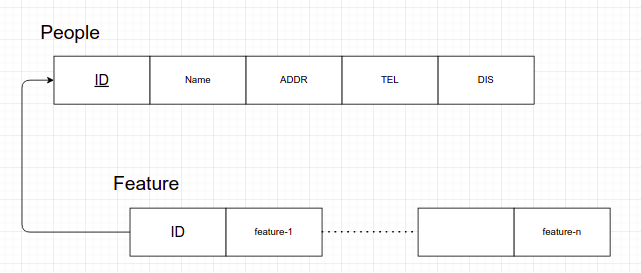
\includegraphics[width=120mm,height=30mm]{fig/24.png}
			%\caption{color histogram similarity measure }
			%\label{color histogram similarity measure}
		\end{figure}
		\begin{figure}[H]
			\centering
			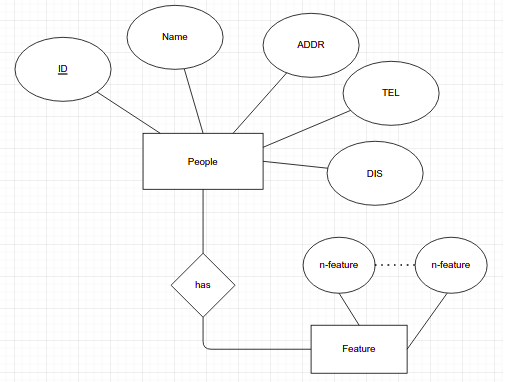
\includegraphics[width=120mm,height=30mm]{fig/25.png}
			%\caption{color histogram similarity measure }
			%\label{color histogram similarity measure}
		\end{figure}
	\end{frame}
	
	
	%------------------------------------------------
	
	\begin{frame}
		\frametitle{References}
		\footnotesize{
			\begin{thebibliography}{99} % Beamer does not support BibTeX so references must be inserted manually as below
				\bibitem[CSE 576 ]{p1} CSE 576 
				\newblock washington.edu
				\newblock \emph{courses.cs.washington.edu/courses/cse576/19s/notes/}
			\end{thebibliography}
		}
	\end{frame}
	
	%------------------------------------------------
	
	\begin{frame}
		\Huge{\centerline{The End}}
	\end{frame}
	
	%----------------------------------------------------------------------------------------
	
\end{document} 